\subsection{Riepilogo}
\subsubsection{Ore totali}

\paragraph{Prospetto orario}
Vengono riportate successivamente le ore totali del progetto, comprese di ore di investimento:

{

\rowcolors{2}{azzurro2}{azzurro3}

\centering
\renewcommand{\arraystretch}{1.8}
\begin{longtable}{C{4cm} C{1cm} C{1cm} C{1cm} C{1cm} C{1cm} C{1cm} C{2cm}}

\rowcolor{azzurro1}
\textbf{Nominativo} &
\textbf{RE}&
\textbf{AM}&
\textbf{AN}&
\textbf{PT}&
\textbf{PR}&
\textbf{VE}&
\textbf{Ore totali}\\
\endhead

\MB & 15 & 14 & 12 & 31 & 28 & 37 & 137 \\
\VAS & 11 & 24 & 15 & 16 & 29 & 42 & 137 \\
\FD & 10 & 18 & 12 & 23 & 28 & 46 & 137 \\
\NM & 10 & 25 & 11 & 16 & 29 & 46 & 137 \\
\SB & 10 & 25 & 12 & 18 & 28 & 44 & 137 \\
\GB & 12 & 14 & 22 & 15 & 34 & 40 & 137 \\
\MDI & 10 & 12 & 24 & 28 & 25 & 38 & 137 \\
\textbf{Ore Totali} & 78 & 132 & 108 & 147 & 201 & 293 & 959 \\

\rowcolor{white}
\caption{Distribuzione oraria totale}\\
\rowcolor{azzurro1}
\end{longtable}
}
\newpage
Il seguente istogramma riassume i dati ottenuti:

\begin{figure}[H]
\centering
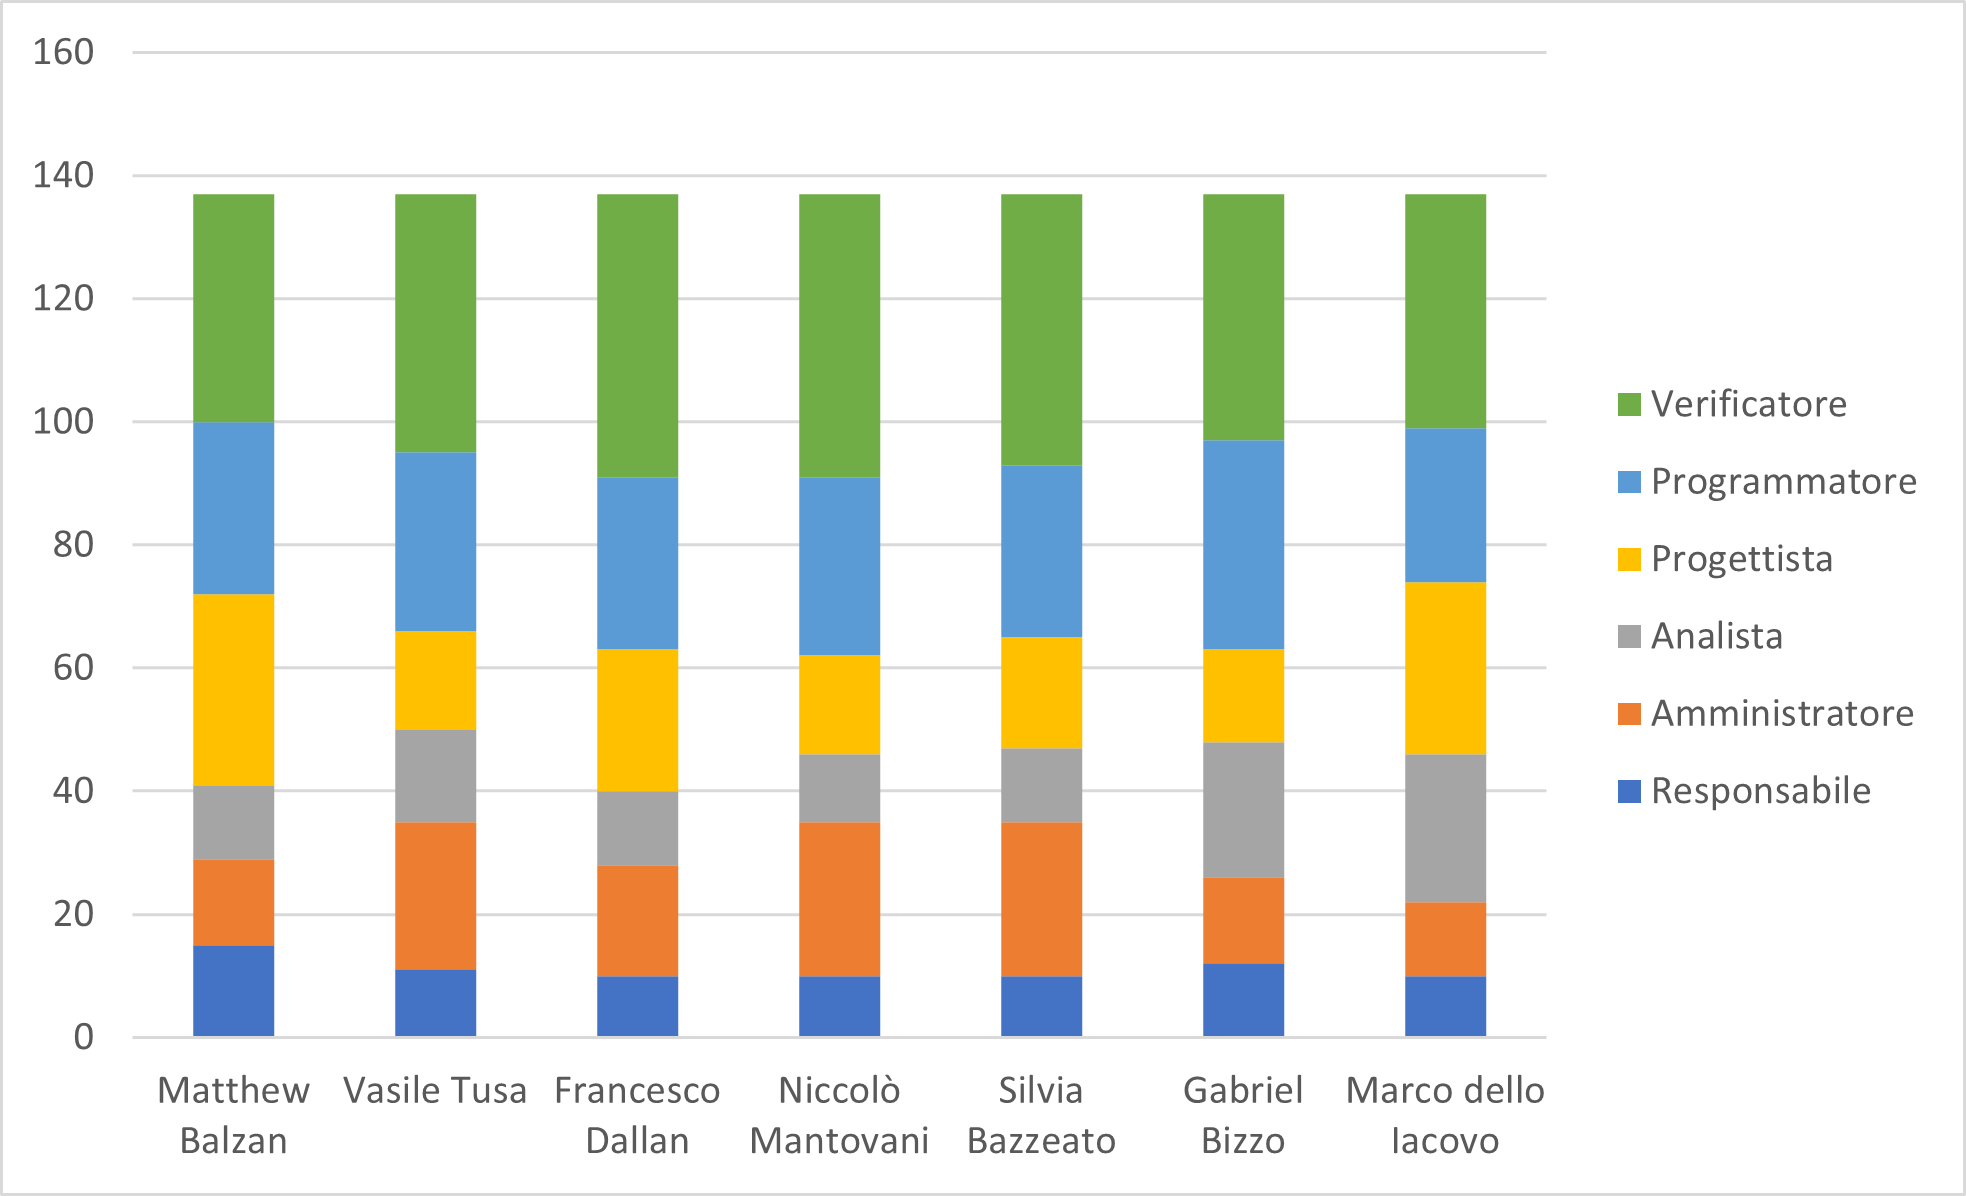
\includegraphics[scale=0.90]{res/Preventivo/Img/istogramma_totale}\\
\caption{Istogramma della ripartizione di ore totali}
\end{figure}


\paragraph{Prospetto economico}

Vengono riportati i costi da affrontare durante l'intero progetto:

{

\rowcolors{2}{azzurro2}{azzurro3}

\centering
\renewcommand{\arraystretch}{1.8}
\begin{longtable}{C{3cm} C{1cm} C{2cm} }
\rowcolor{azzurro1}
\textbf{Ruolo} &
\textbf{Ore}&
\textbf{Costo}\\
\endhead

\textit{Responsabile} & 78 & 2340\euro{} \\
\ammProg & 132 & 2640\euro{} \\
\analProg & 108 & 2700\euro{} \\
\progetProg & 147 & 3234\euro{} \\
\programProg & 201 & 3015\euro{} \\
\verifProg & 293 & 4395\euro{} \\
\textbf{Totale} & 959 & 18324\euro{} \\
\rowcolor{white}
\caption{Prospetto dei costi per ruolo per l'intero progetto}

\end{longtable}

}
\newpage
Il seguente areogramma riassume i dati ottenuti:

\begin{figure}[H]
\centering
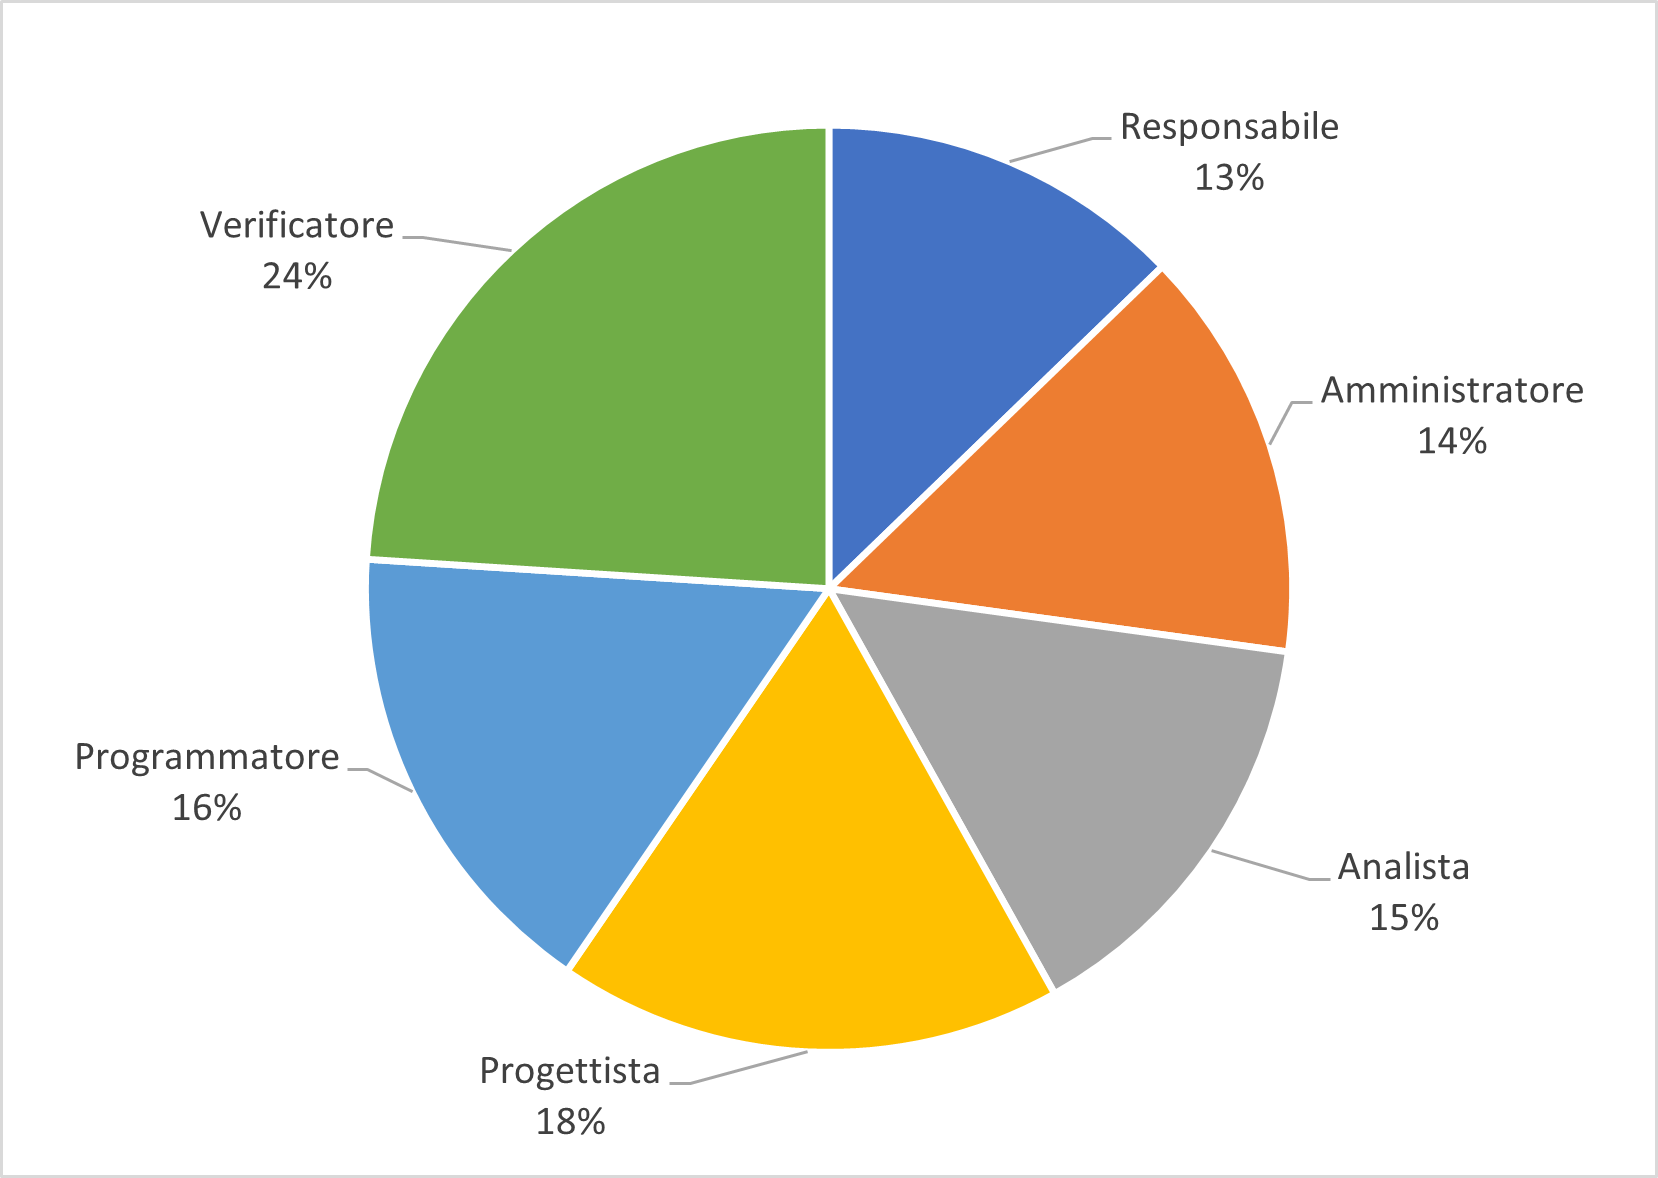
\includegraphics[scale=0.90]{res/Preventivo/Img/areogramma_totale}\\
\caption{Areogramma della distribuzione economica totale}
\end{figure}








\subsubsection{Ore rendicontate}
\paragraph{Prospetto orario}
Vengono riportate successivamente le ore totali rendicontate del progetto:

{

\rowcolors{2}{azzurro2}{azzurro3}

\centering
\renewcommand{\arraystretch}{1.8}
\begin{longtable}{C{4cm} C{1cm} C{1cm} C{1cm} C{1cm} C{1cm} C{1cm} C{2cm}}

\rowcolor{azzurro1}
\textbf{Nominativo} &
\textbf{RE}&
\textbf{AM}&
\textbf{AN}&
\textbf{PT}&
\textbf{PR}&
\textbf{VE}&
\textbf{Ore totali}\\
\endhead

\MB & 0 & 14 & 0 & 31 & 28 & 29 & 102 \\
\VAS & 11 & 6 & 10 & 16 & 29 & 30 & 102 \\
\FD & 0 & 10 & 7 & 23 & 28 & 34 & 102 \\
\NM & 10 & 5 & 6 & 16 & 29 & 36 & 102 \\
\SB & 10 & 7 & 5 & 18 & 28 & 34 & 102 \\
\GB & 12 & 14 & 0 & 15 & 34 & 27 & 102 \\
\MDI & 10 & 12 & 0 & 28 & 25 & 27 & 102 \\
\textbf{Ore Totali} & 53 & 68 & 28 & 147 & 201 & 217 & 714 \\

\rowcolor{white}
\caption{Distribuzione delle ore rendicontate}\\
\rowcolor{azzurro1}
\end{longtable}
}
\newpage
Il seguente istogramma riassume i dati ottenuti:

\begin{figure}[H]
\centering
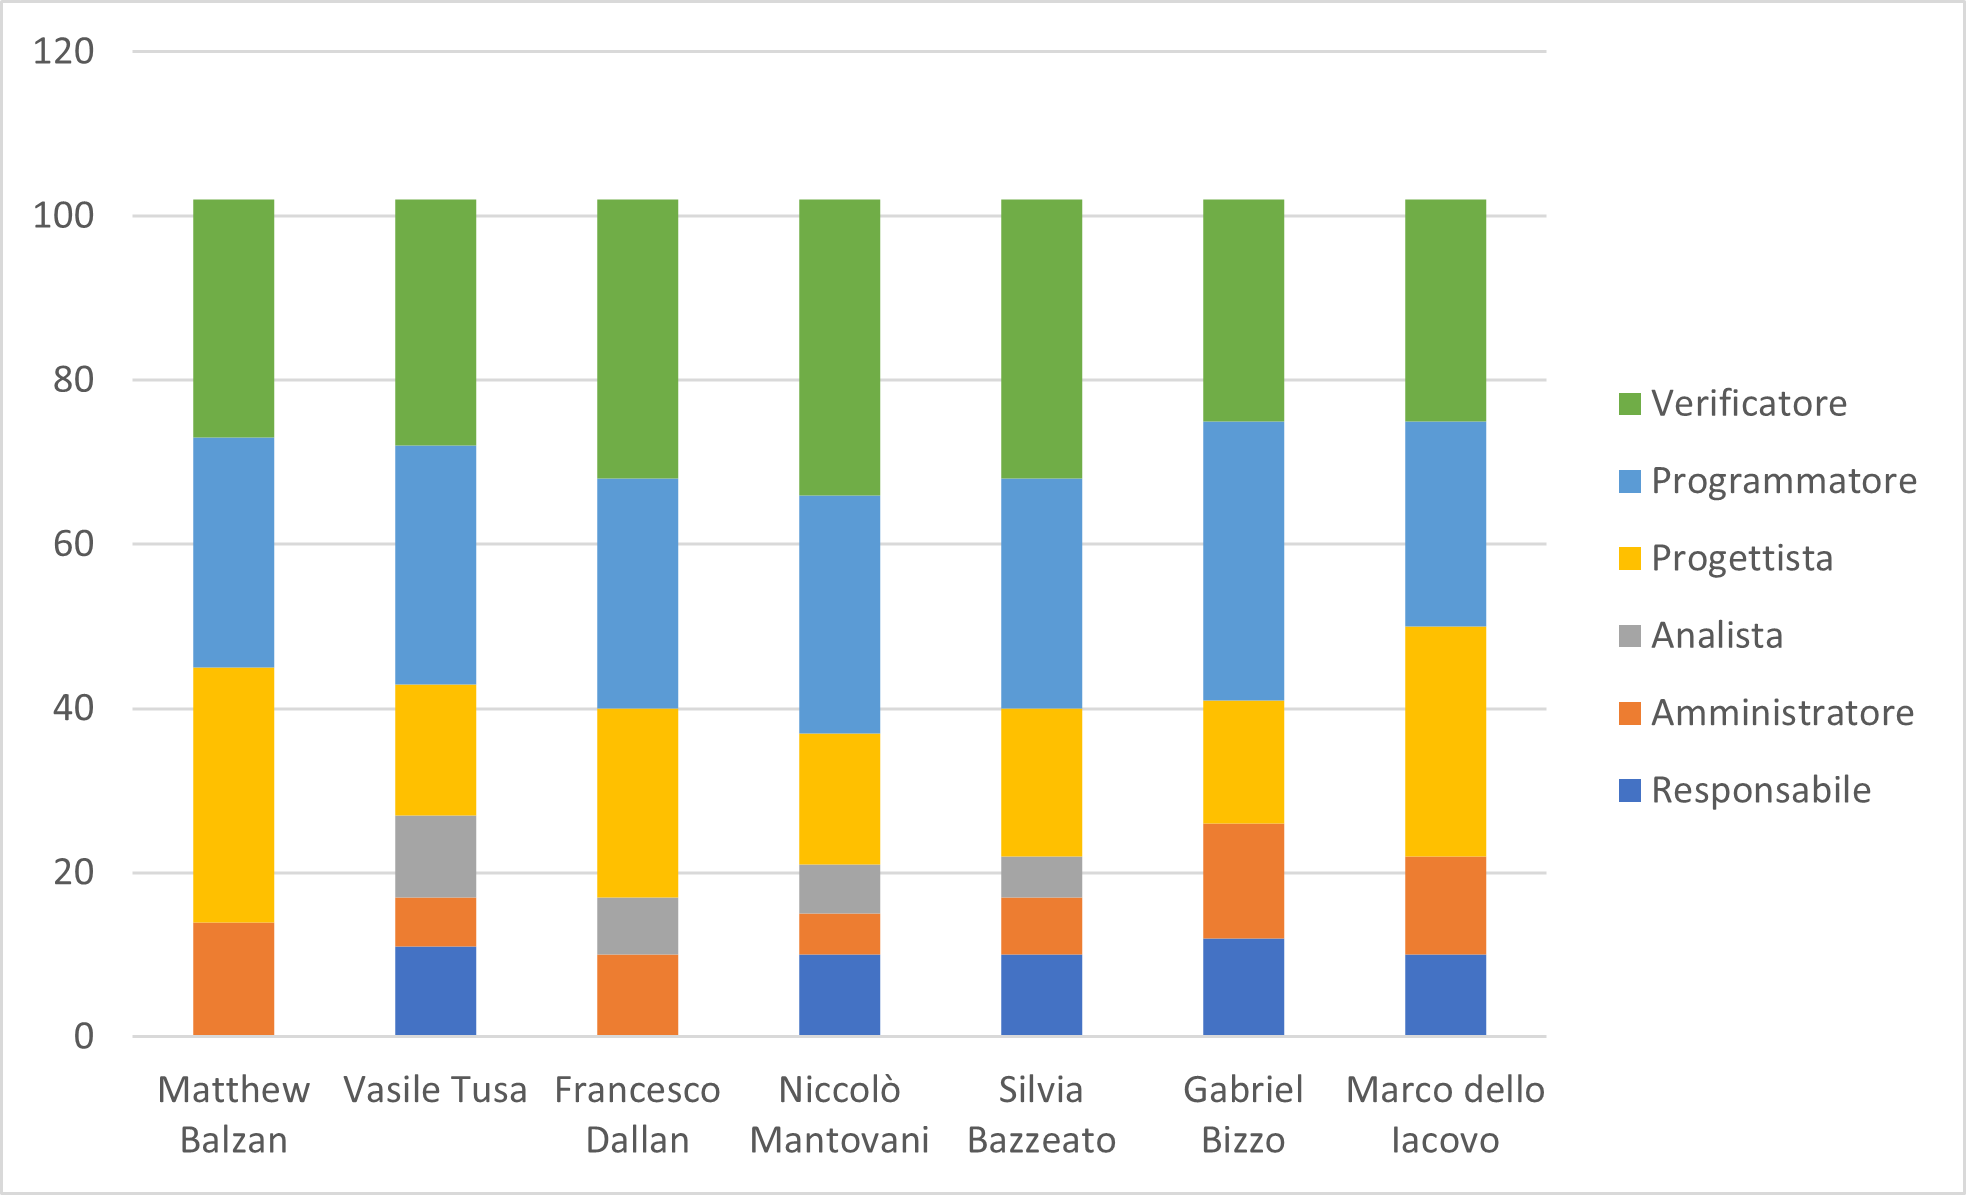
\includegraphics[scale=0.90]{res/Preventivo/Img/istogramma_rendicontato}\\
\caption{Istogramma della ripartizione di ore rendicontate}
\end{figure}


\paragraph{Prospetto economico}

Vengono riportati i costi da affrontare durante il periodo rendicontato:

{

\rowcolors{2}{azzurro2}{azzurro3}

\centering
\renewcommand{\arraystretch}{1.8}
\begin{longtable}{C{3cm} C{1cm} C{2cm} }
\rowcolor{azzurro1}
\textbf{Ruolo} &
\textbf{Ore}&
\textbf{Costo}\\
\endhead

\textit{Responsabile} & 53 & 1590\euro{} \\
\ammProg & 68 & 1360\euro{} \\
\analProg & 28 & 700\euro{} \\
\progetProg & 147 & 3234\euro{} \\
\programProg & 201 & 3015\euro{} \\
\verifProg & 217 & 3255\euro{} \\
\textbf{Totale} & 714 & 13154\euro{} \\
\rowcolor{white}
\caption{Prospetto dei costi per ruolo per il periodo rendicontato}

\end{longtable}

}
\newpage
Il seguente areogramma riassume i dati ottenuti:

\begin{figure}[H]
\centering
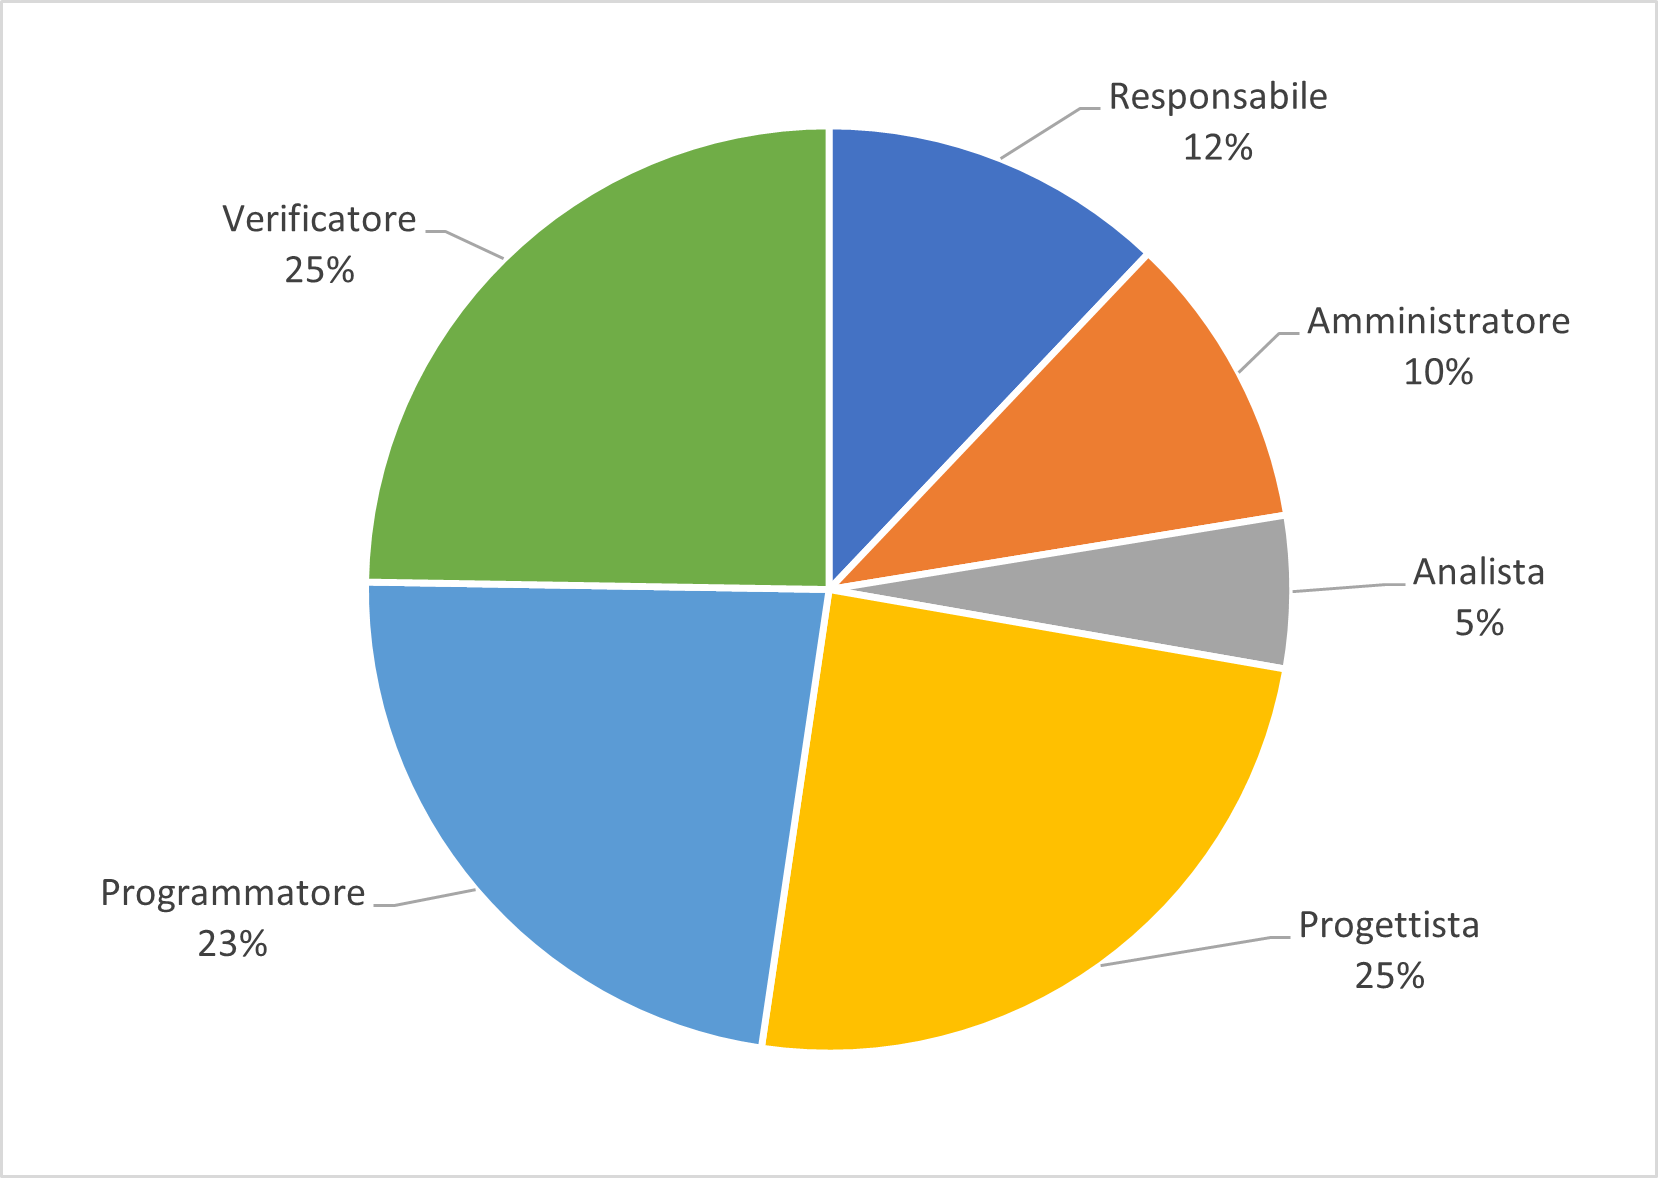
\includegraphics[scale=0.90]{res/Preventivo/Img/areogramma_rendicontato}\\
\caption{Areogramma della distribuzione economica rendicontata}
\end{figure}